\item A right-angled prism of refractive index $\mu_1$ is placed in a rectangular block of refractive index $\mu_2$, which is surrounded by a medium of refractive index $\mu_3$, as shown in the figure. A ray of light `e' enters the rectangular block at normal incidence. Depending upon the relationships between $\mu_1$, $\mu_2$ and $\mu_3$, it takes one of the four possible paths `ef', `eg', `eh' or `ei'.

\begin{center}
    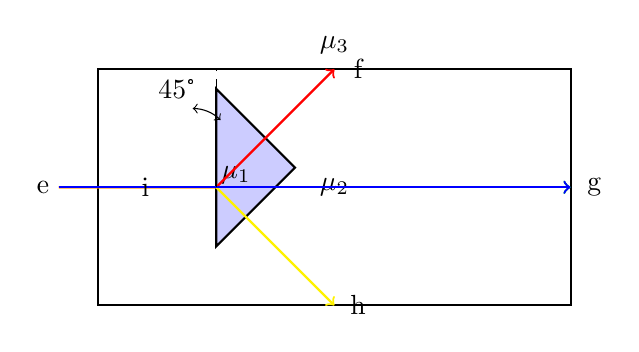
\begin{tikzpicture}
        % Define styles for the different elements in the diagram
        \tikzstyle{prism} = [fill=blue!20, thick]

        % Draw the rectangular block
        \draw[thick] (0,0) rectangle (6,3);
        \node at (3,1.5) {$\mu_2$};

        % Draw the right angle prism inside the rectangular block
        \draw[prism] (1.5,0.75) -- ++(45:1.414) -- ++(135:1.414) -- cycle;
        \node at (1.75,1.65) {$\mu_1$};

        % Draw path 'ef' (e to f)
        \draw[->, thick, red] (-0.5,1.5) -- (1.5,1.5) -- (3,3);
        \node at (3.3,3) {f};

        % Draw path 'eg' (e to g)
        \draw[->, thick, green] (-0.5,1.5) -- (1.5,1.5) -- (6,1.5);
        \node at (6.3,1.5) {g};

        % Draw path 'eh' (e to h)
        \draw[->, thick, yellow] (-0.5,1.5) -- (1.5,1.5) -- (3,0);
        \node at (3.3,0) {h};

        % Draw path 'ei' (e to i)
        \draw[->, thick, blue] (-0.5,1.5) -- (6,1.5);
        \node at (-0.7,1.5) {e};

        % Draw normal line and incidence angle
        \draw[dashed] (1.5,1.5) -- (1.5,3);
        \draw[<->] (1.2,2.5) arc (90:45:0.5);
        \node at (1,2.75) {45°};
        \node at (0.6,1.5) {i};

        % Draw the medium around the rectangular block
        \node at (3,3.3) {$\mu_3$};

    \end{tikzpicture}
\end{center}

\begin{center}
    \renewcommand{\arraystretch}{2}
    \begin{table}[h]
        \centering
        \begin{tabular}{p{0.25cm}p{8cm}|p{0.25cm}p{5cm}}
        \hline
        & List I & & List II \\
        \hline
        (P)& $e \rightarrow f$ & (1) & $\mu_1 > \sqrt{2} \mu_2$\\
        (Q)& $e \rightarrow g$ & (2) & $\mu_2 > \mu_1 \text{ and/or } \mu_2 > \mu_3$\\
        (R)& $e \rightarrow h$ & (3) & $\mu_1 = \mu_2$\\
        (S)& $e \rightarrow i$ & (4) & $\mu_2 < \mu_1 < \sqrt{2} \mu_2 \text{ and/or } \mu_2 > \mu_3$\\
        \hline
        \end{tabular}
    \end{table}
\end{center}

\begin{tasks}(2)
    \task P $\rightarrow$ 2, Q $\rightarrow$ 3, R $\rightarrow$ 1, S $\rightarrow$ 4
    \task P $\rightarrow$ 1, Q $\rightarrow$ 2, R $\rightarrow$ 4, S $\rightarrow$ 3
    \task P $\rightarrow$ 4, Q $\rightarrow$ 1, R $\rightarrow$ 2, S $\rightarrow$ 3
    \task P $\rightarrow$ 2, Q $\rightarrow$ 3, R $\rightarrow$ 4, S $\rightarrow$ 1
\end{tasks}